\chapter{\label{ax:b-hybrid_reactivation_il_caos_delle_sfere}Case study. Hybrid Reactivation \textit{Il caos delle sfere}}

The reactivation of Carlo De Pirro’s interactive installation \textit{Il caos delle sfere} has been an important case study in this research project. This process involved migrating the installation’s computer-based part to newer, more streamlined, and performative technologies. Although this reactivation underwent a digital-to-digital migration — an interesting contrast to the more common analogue-to-digital migration, as discussed in Appendix~\ref{ax:a-michele_sambin_videoloop} with the \textit{videoloop} reactivation — we refer to it as a hybrid reactivation because certain parts of the installation required a philological approach.\\
This case study was important for testing the \textit{Multilevel Dynamic Conservation} (MDC) and CATTA reactivation workflow and their application in the Graph Database Neo4j.

\section{Objectives}
The main objectives of this case study, in addition to the application, testing and refinement of the systems introduced in Chapter~\ref{ch:3-mdc_model-reactivation_workflow-instruction_template}, are:
\begin{enumerate}
    \item to explore the role of interdisciplinary collaboration in developing, supporting, and reactivating artworks;
    \item to apply reactivation through software archaeology, hardware repairs, porting, and digital-to-digital migration;
    \item to explore how audiences interact with installations;
    \item to create a Neo4j database according to the MDC model–see Chapter~\ref{ch:4-madc_model_application} for more details.
\end{enumerate}

\section{Introduction}
Carlo De Pirro was an Italian composer who began his career working with instrumental and electroacoustic music, later expanding into musical theatre and interactive installations. Among his important works are those created using the Yamaha Disklavier, an automatic player piano, which became a key part of his creative expression. With this particular instrument, the composer explored the possibilities of playing increasingly complex scores, which are impossible for a human performer to execute. He used this instrument in various settings: for chamber music compositions like \textit{Di vento e cristallo} (1998) for Disklavier and flute; for electroacoustic pieces, such as \textit{Rifr-azioni} (1997) for accordion processed via MARS and Disklavier; for orchestral compositions, including one of his last works \textit{Addio!} (2007); for theatrical productions like\textit{ Generatore di Ombre} (2001); and installations such as \textit{Il caos delle sfere} (1999) and \textit{Il tempo sospeso} (2007) (in Figure~\ref{fig:ab-iltemposospeso}).

\begin{figure}[!h]
    \centering
    \includegraphics[width=\linewidth]{chapters/appendix/b/image/figb-iltemposospeso.png}
    \caption{Carlo De Pirro’s installation \textit{Il tempo sospeso} (2007), for Disklavier and electroacoustic processing, installed in Palazzo della Ragione in Padova in 2007.}
    \label{fig:ab-iltemposospeso}
\end{figure}

Another significant aspect of De Pirro's career was his collaboration with the Centro di Sonologia Computazionale (CSC) starting in the early 1980s. In addition to his work with MARS–a processor developed by IRIS in collaboration with CSC–his partnership with the laboratory was crucial in the creation of musical installations during the 1990s and 2000s. These include not only \textit{Il caos delle sfere} (1999) but also installations like those created for the 2002 EXPO in Switzerland; \textit{Carillion}, which featured an automated carillon made from carpenter tools that played compositions by De Pirro; and \textit{La casetta delle immagini}, an immersive and interactive room where the audience's movements controlled the lights, colours and the sound diffusion inside.\\
From the installations emerged the CAPIRE project (\textit{CArlo de PIrro: Restoring an Experience}), which ran from 2009 (a year after De Pirro's death) to 2014. This project aimed to reactivate some of Carlo De Pirro's installations, leading to the development of the first version of the \textit{Multilevel Dynamic Conservation} model \cite{bressan2009preserving, bressan2014challenge} presented in this thesis in Chapter~\ref{ch:3-mdc_model-reactivation_workflow-instruction_template}.

\subsection*{Il caos delle sfere}
The work \textit{Il Caos delle Sfere: anche tu musicista con 500 lire} (translated into English \textit{The sphere’s chaos: Be a Musician with 500 Italian Lire}) premiered on 9 June 1999 at the Biennale of Young Artists of Europe and the Mediterranean in Rome. It was installed several times in Italy and Europe until 2004.\\
The main musical component of this installation is the Disklavier Yamaha, and it was the first attempt to use the instrument within an art installation. In this case, the instrument was combined with a pinball machine as an interactive component.\\
The primary purpose of this installation was to bring contemporary music and musical research to the general public, and a pinball machine was one of the most popular games at the time. In addition, the electronic pinball turned out to be an interesting tool for creating a musical structure: the wide variety of possible interactions could make each performance unique, besides combining sight, hearing and touch. Choosing a specific pinball model over a generic one was also relevant for this installation. In fact, the selected model is the 1992 \textit{Creature of the Black Lagoon}, the first one to add a story with different goals to achieve. This feature allowed the composer to create a more intricate relationship between the game and the music. Instead of simply matching each object hit by the ball with a single sound, the Disklavier plays increasingly elaborate musical sequences level after level following the game's progress. A better player will be rewarded with a longer and more complex performance while remaining able to master the changes during the gameplay. The artistic idea behind the installation was to make a player able to govern the chaos, i.e. the fact that a pinball game can be very random so that it can reach a state where the game is more controlled and predictable: this is reflected in the way the musical performance evolves.\\
The composer realised the installation together with a research group of the CSC, composed by Nicola Orio and Paolo Cogo, in Figure~\ref{fig:ab-ilcaosdellesfere-group01}. The group developed a dedicated software to implement the communication between the pinball (the interaction side) and the Disklavier (the playback side). The pinball machine sends the signal of its main components (switches to track targets hit by the ball and lights to monitor the game level) to a computer through a parallel port. The software interprets the signal and controls the Disklavier through a MIDI communication: it can choose between forty-three MIDI sequences, a selection of all the sequences written by De Pirro, elaborated further by the so-called \textit{Controlled Refractions} (computer-generated musical gestures intertwined with real-time performance, studied in those years by the composer together with Nicola Orio at the CSC) \cite{orio1998controlled}. The graphical user interface was minimal and only designed for testing purposes. Without any feedback from the computer, the player could explore the relations between the game and the music and get surprised by hitting a different spot or reaching a new level.

\begin{figure}[!h]
    \centering
    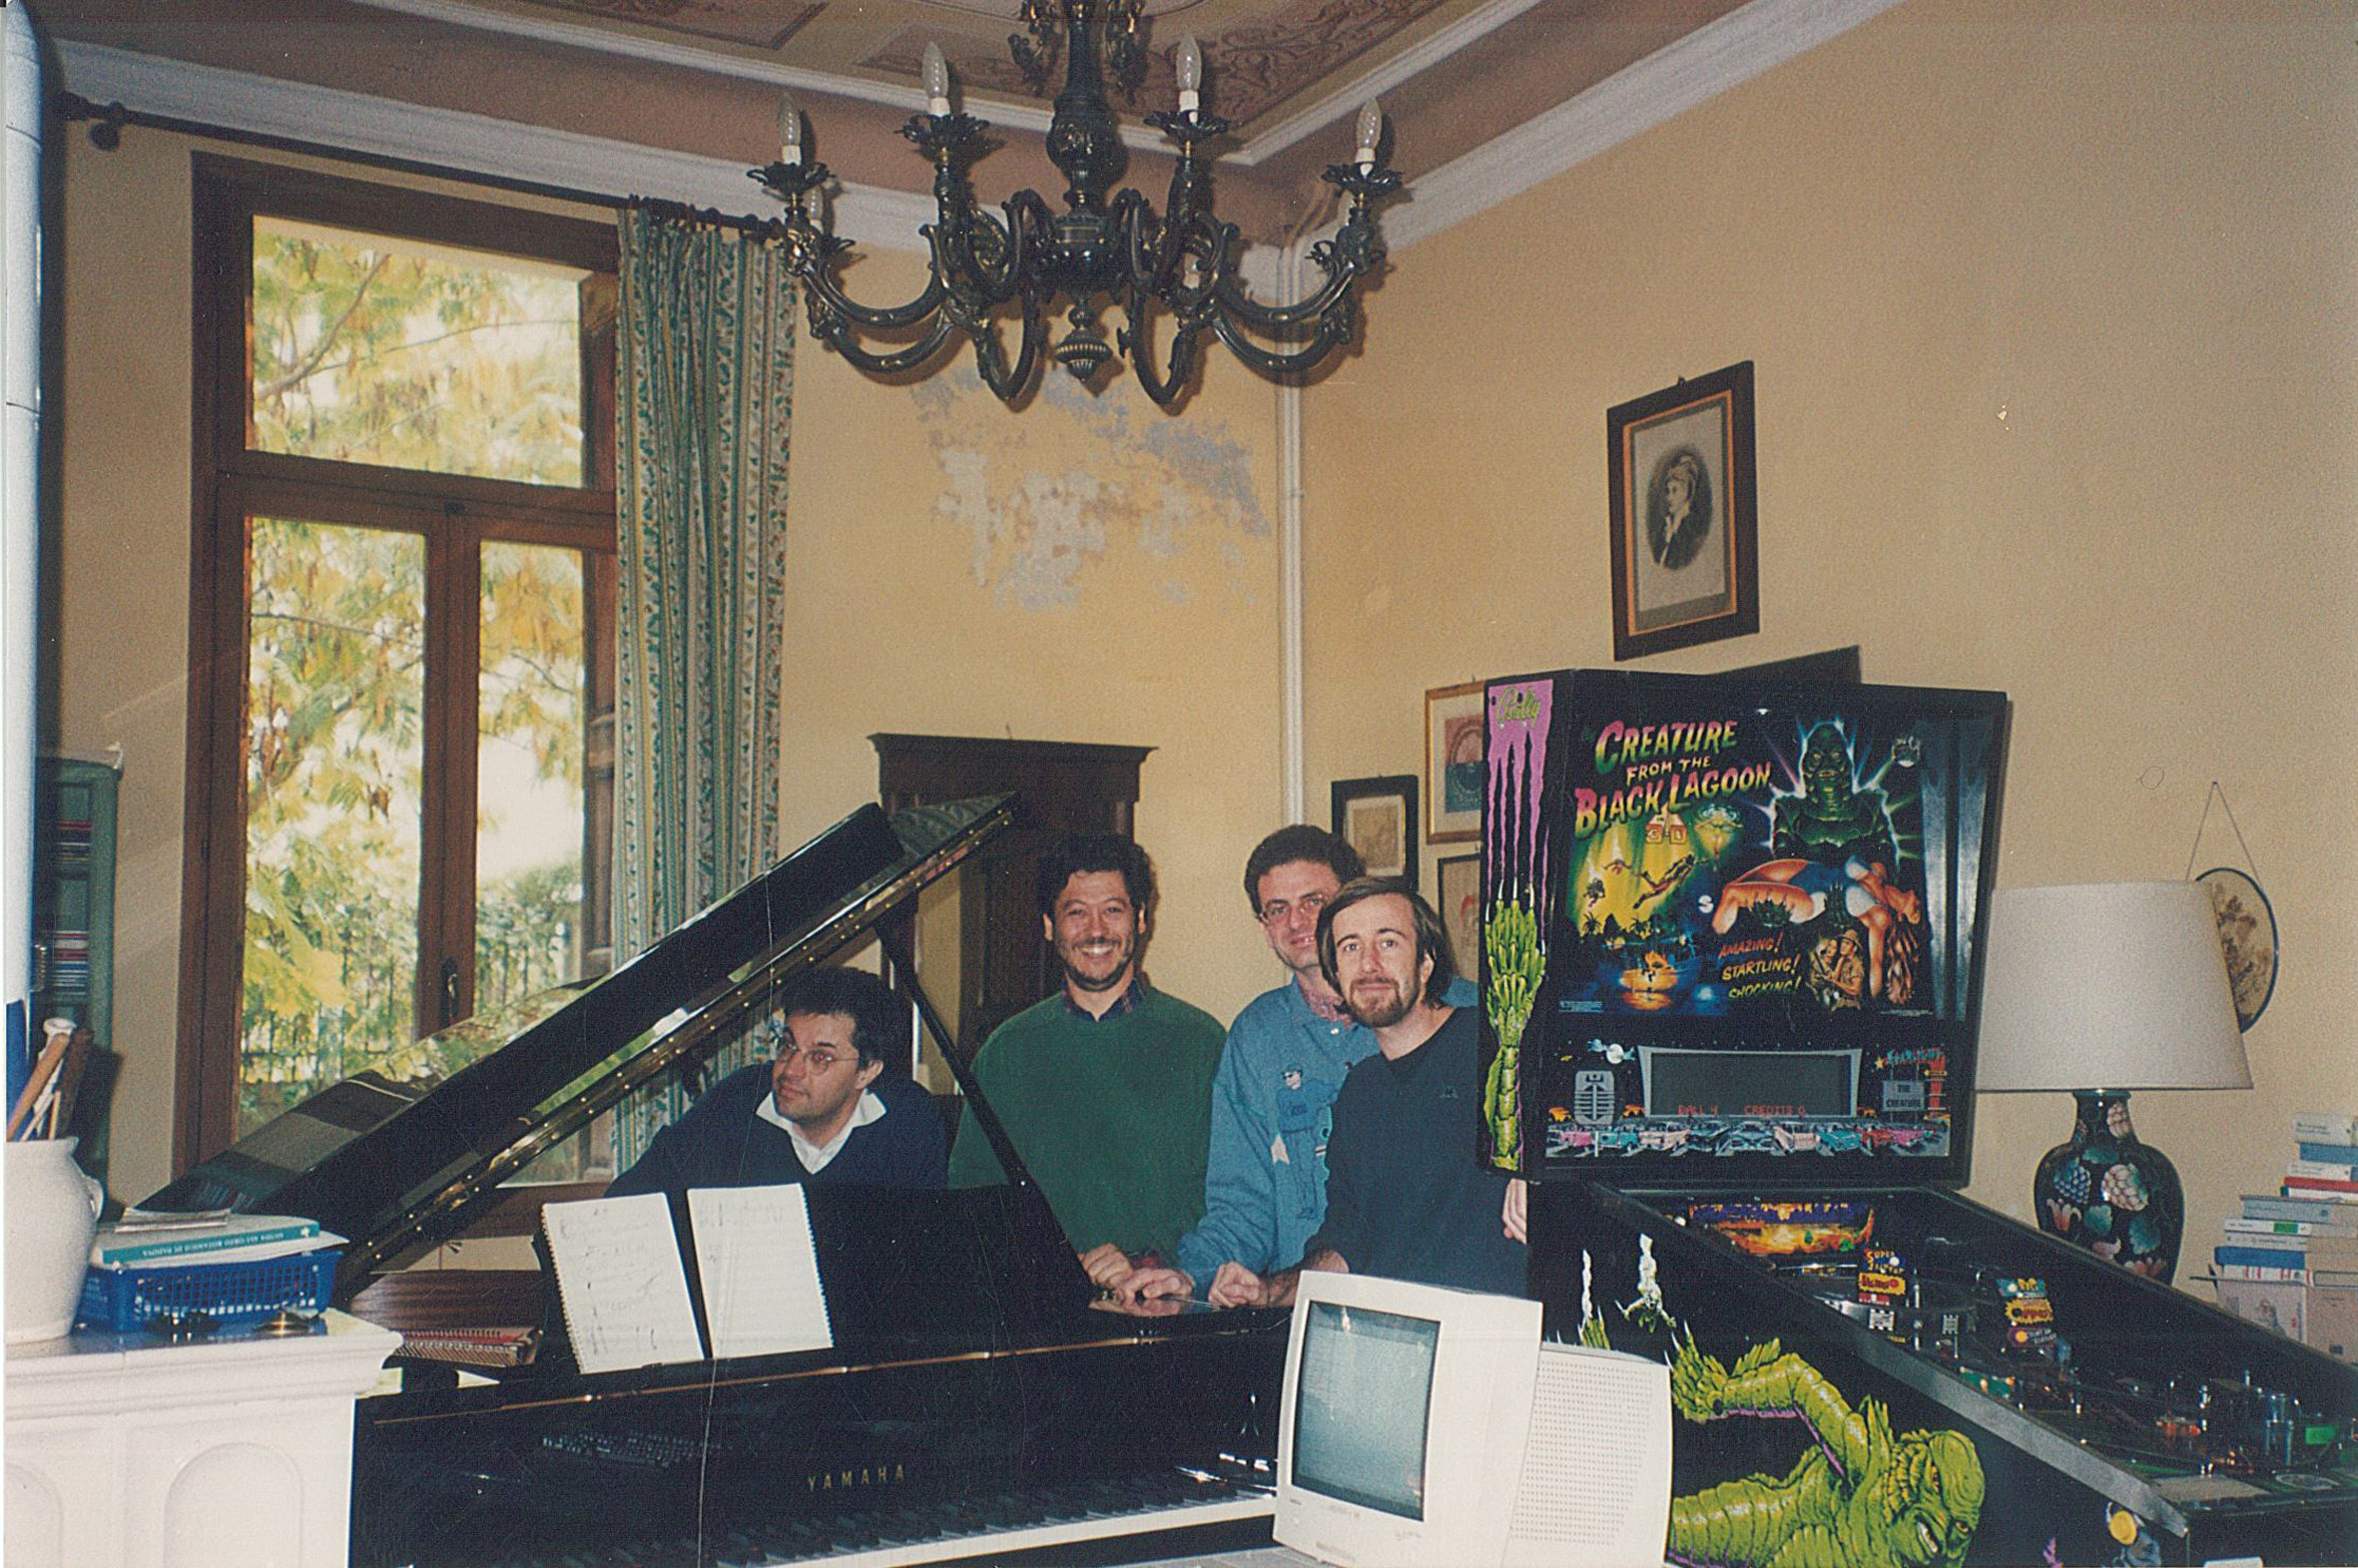
\includegraphics[width=\linewidth]{chapters/appendix/b/image/figb-ilcaosdellesfere-group01.jpg}
    \caption{The research group that developed \textit{Il Caos delle sfere} in 1999 at Carlo De Pirro’s home. From left to right: Veniero Rizzardi, Carlo De Pirro, Paolo Cogo, and Nicola Orio. On the left is the Disklavier, and on the right is the Pinball \textit{Creature of the Black Lagoon}.}
    \label{fig:ab-ilcaosdellesfere-group01}
\end{figure}

\section{Reactivation}
The reactivation and preservation processes occurred at the CSC lab between March 2022 and February 2023. The research project was carried out by an interdisciplinary research group composed of engineers, electronic music researchers, a time-based media art researcher, and an audio-visual preservation expert (Figure~\ref{fig:ab-ilcaosdellesfere-group02} shows part of the research group). The assistance of some of the original installation technicians was essential since critical parts of the installation were left undocumented. Unfortunately, the project could not rely on the composer's participation since he passed away in 2008.

\begin{figure}[!h]
    \centering
    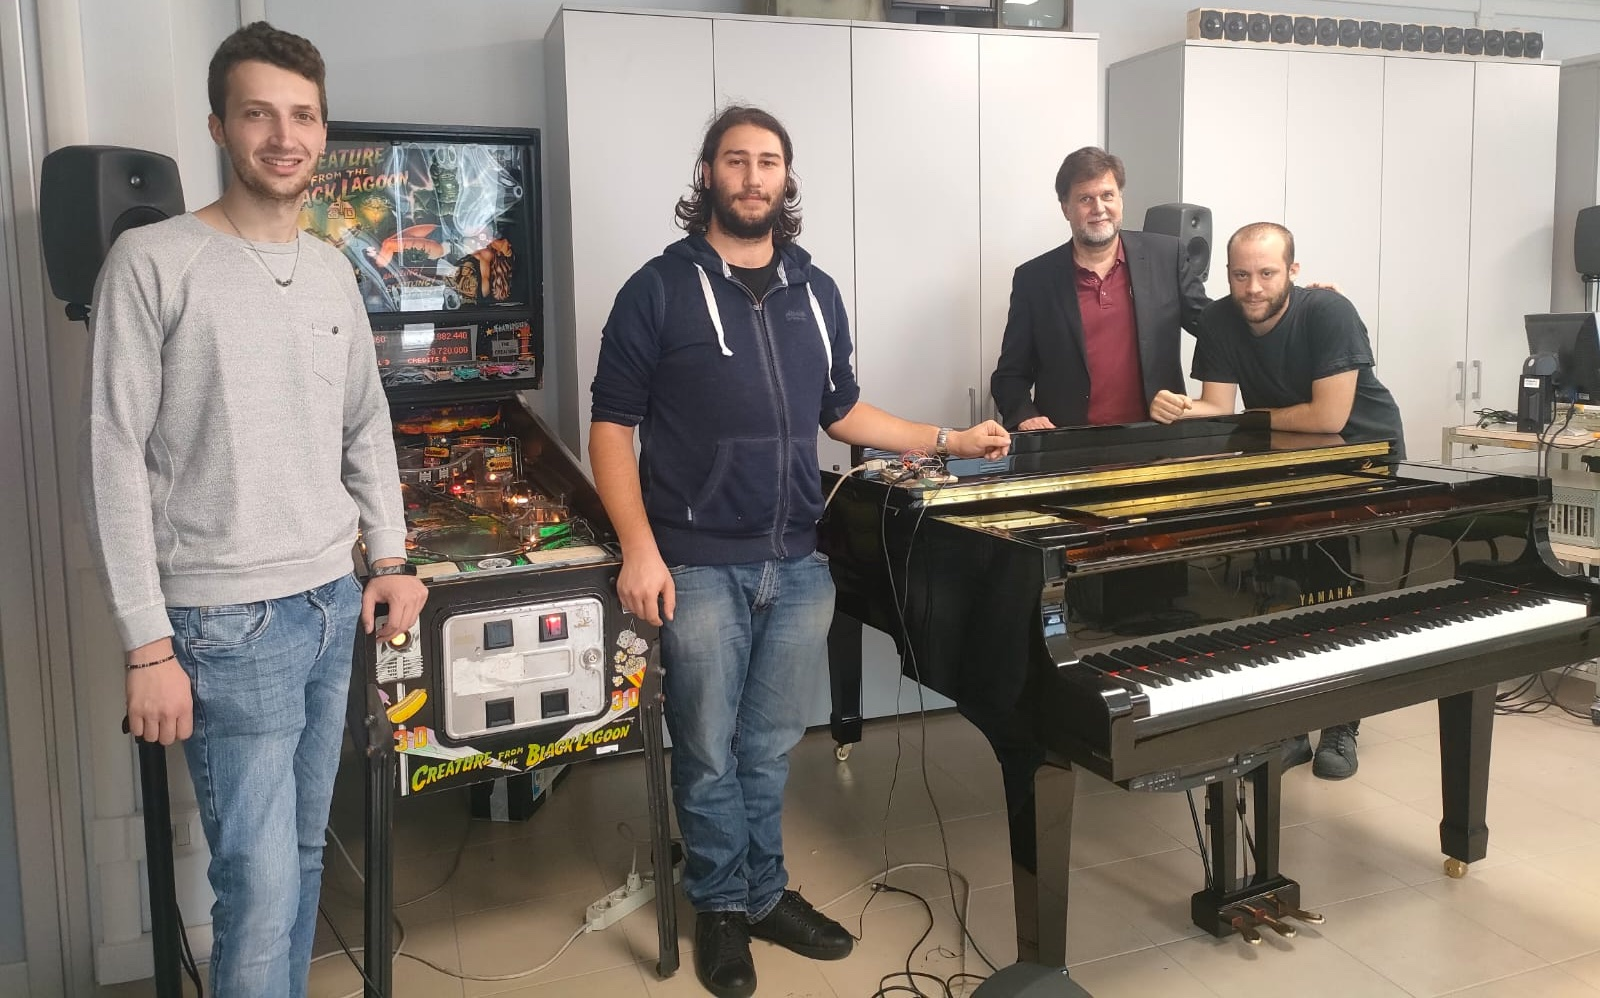
\includegraphics[width=\linewidth]{chapters/appendix/b/image/figb-ilcaosdellesfere-group02.jpg}
    \caption{Part of the research group that worked on the reactivation of \textit{Il Caos delle sfere} between 2022 and 2023 1999 at Centro di Sonologia Computazionale (CSC). From left to right: Luca Zecchinato (engineering master thesis student), Mattia Pizzato (from SaMPL's Conservatory of Padua), Sergio Canazza (CSC Director), and the author of the text.}
    \label{fig:ab-ilcaosdellesfere-group02}
\end{figure}

\subsection*{Collection}
The first step was assembling the \textit{Iteration Files} (IFs) from past installation exhibitions. Gathering almost all the original installation \textit{bit}s (pinball machine and original computer) was straightforward as all of them were being preserved at the CSC. The Disklavier was borrowed from the Conservatory of Padua's Sound and Music Processing Lab (SaMPL). Nevertheless, collecting data, i.e. mappings and the necessary technical and operative instructions for the activation, was challenging. During its many representations, the research team and the composer kept updating the installation to fit the exhibition’s context best and refine and improve the final musical experience. For example, the software was developed with a trial-and-error approach, with almost no comments included (as witnessed by Nicola Orio). More than ten versions of the same source code were developed, introducing uncertainty about the proper version to consider. The same goes for instructions on how to make the physical part of the system communicate. The experience documentation collection consisted mainly of photos and videos of the installation being performed. Besides the existing documentation, new resources were produced. The oral history resources obtained from some of the technicians who worked at one of the representations of the installation (Nicola Orio, Sergio Canazza, and Antonio Rodà) were very useful.

\subsection*{Assessment}
Given the physical and logical parts and the related documentation, the next step was to produce a high-level description of the artwork as a whole. We created conceptual (Figure~\ref{fig:ab-mapping-conceptual}) and physical implementation (Figure~\ref{fig:ab-mapping-physical}) mappings to better address the \textit{bit}s' condition evaluations. The goal was to analyse the overall performative system’s rehabilitation, fielding the issues of the technological migration and recovery of analogue tools.\\ 
In Figure~\ref{fig:ab-mapping-conceptual}, we explain the interaction system from the perspective of the audience's experience, focusing on how their actions trigger responses in the system. \\
The physical implementation in Figure~\ref{fig:ab-mapping-physical} shows how the different components (\textit{bit}s) of the interactive installation are organised, each serving a specific function:
\begin{itemize}
    \item \textit{Interaction}. This is the role of the pinball machine, which generates in-game data signals. These signals are used to select the musical sequences that will be played.
    \item \textit{Communication}. This is the role of the computer, which connects the pinball machine to the Disklavier. It translates the real-time signals from the pinball (received through the parallel port) into corresponding musical sequences, sending them as MIDI events to the Disklavier (via the MIDI out port).
    \item \textit{Playback}. This is the role of the Disklavier. The automatic piano plays musical sequences in real-time based on the player's actions, providing the game with real-time experiential feedback.
\end{itemize}
The pinball machine is the part of the artwork where users can directly interact to shape the final musical performance. This pinball machine is modified with a custom-built internal circuit board that sends 31 signals (from sensors and lights) through a 25-pin parallel communication system (Figure~\ref{fig:ab-ilcaosdellesfere-pcb}). Conversely, the Disklavier handles the playback of the musical sequences generated by the interaction. Looking at both the conceptual (Figure~\ref{fig:ab-mapping-conceptual}) and physical implementation (Figure~\ref{fig:ab-mapping-physical}) mappings, we can see that these two elements—the pinball machine and Disklavier—are central to both the idea and the function of the installation. They create an interactive experience between the audience and the artwork. Their unique characteristics further emphasise the importance of these specific components: the pinball machine is themed after \textit{Creature of the Black Lagoon}, with its own story and gameplay mechanics. At the same time, the Disklavier is an automatic acoustic piano. Although alternatives exist, Yamaha models are the most popular and easy to find, making them a practical choice for the installation.\\ 
\begin{figure}[!h]
    \centering
    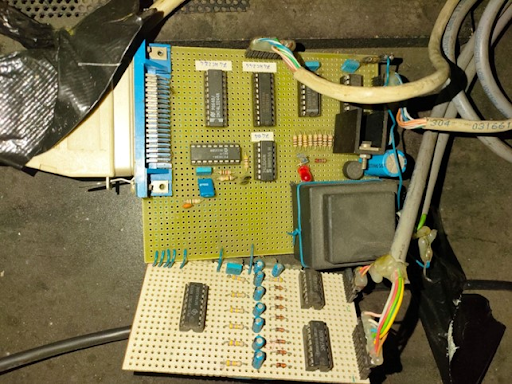
\includegraphics[width=\linewidth]{chapters/appendix/b/image/figb-ilcaosdellesfere-pcb.jpg}
    \caption{shows the pinball’s custom-built internal circuit board, which allows 31 signals from the machine’s sensors and lights to be sent via a parallel port.}
    \label{fig:ab-ilcaosdellesfere-pcb}
\end{figure}
The computer in Figure~\ref{fig:ab-ilcaosdellesfere-computer} is the part of the artwork that makes the pinball and the Disklavier communicate. The original computer is a 1998 Desktop Personal Computer running Windows 1995 with an integral DB25 Parallel Port interface, a Sound card with MIDI interface, and a Graphics card. The computer in the installation represents the subsystem responsible for running the main software (written in C) that processes, generates, and modifies melodic sequences played by the Disklavier based on the actions in the pinball game. Over time, the computer was never updated due to the rapid advancement of technology. This outdated state has made it obsolete and unreliable for public exhibitions, with several parts, like the motherboard slots, graphics card, and DB25 parallel connection, being damaged.
\begin{figure}[h!]
    \centering
    \begin{minipage}[t]{0.48\textwidth}
        \centering
        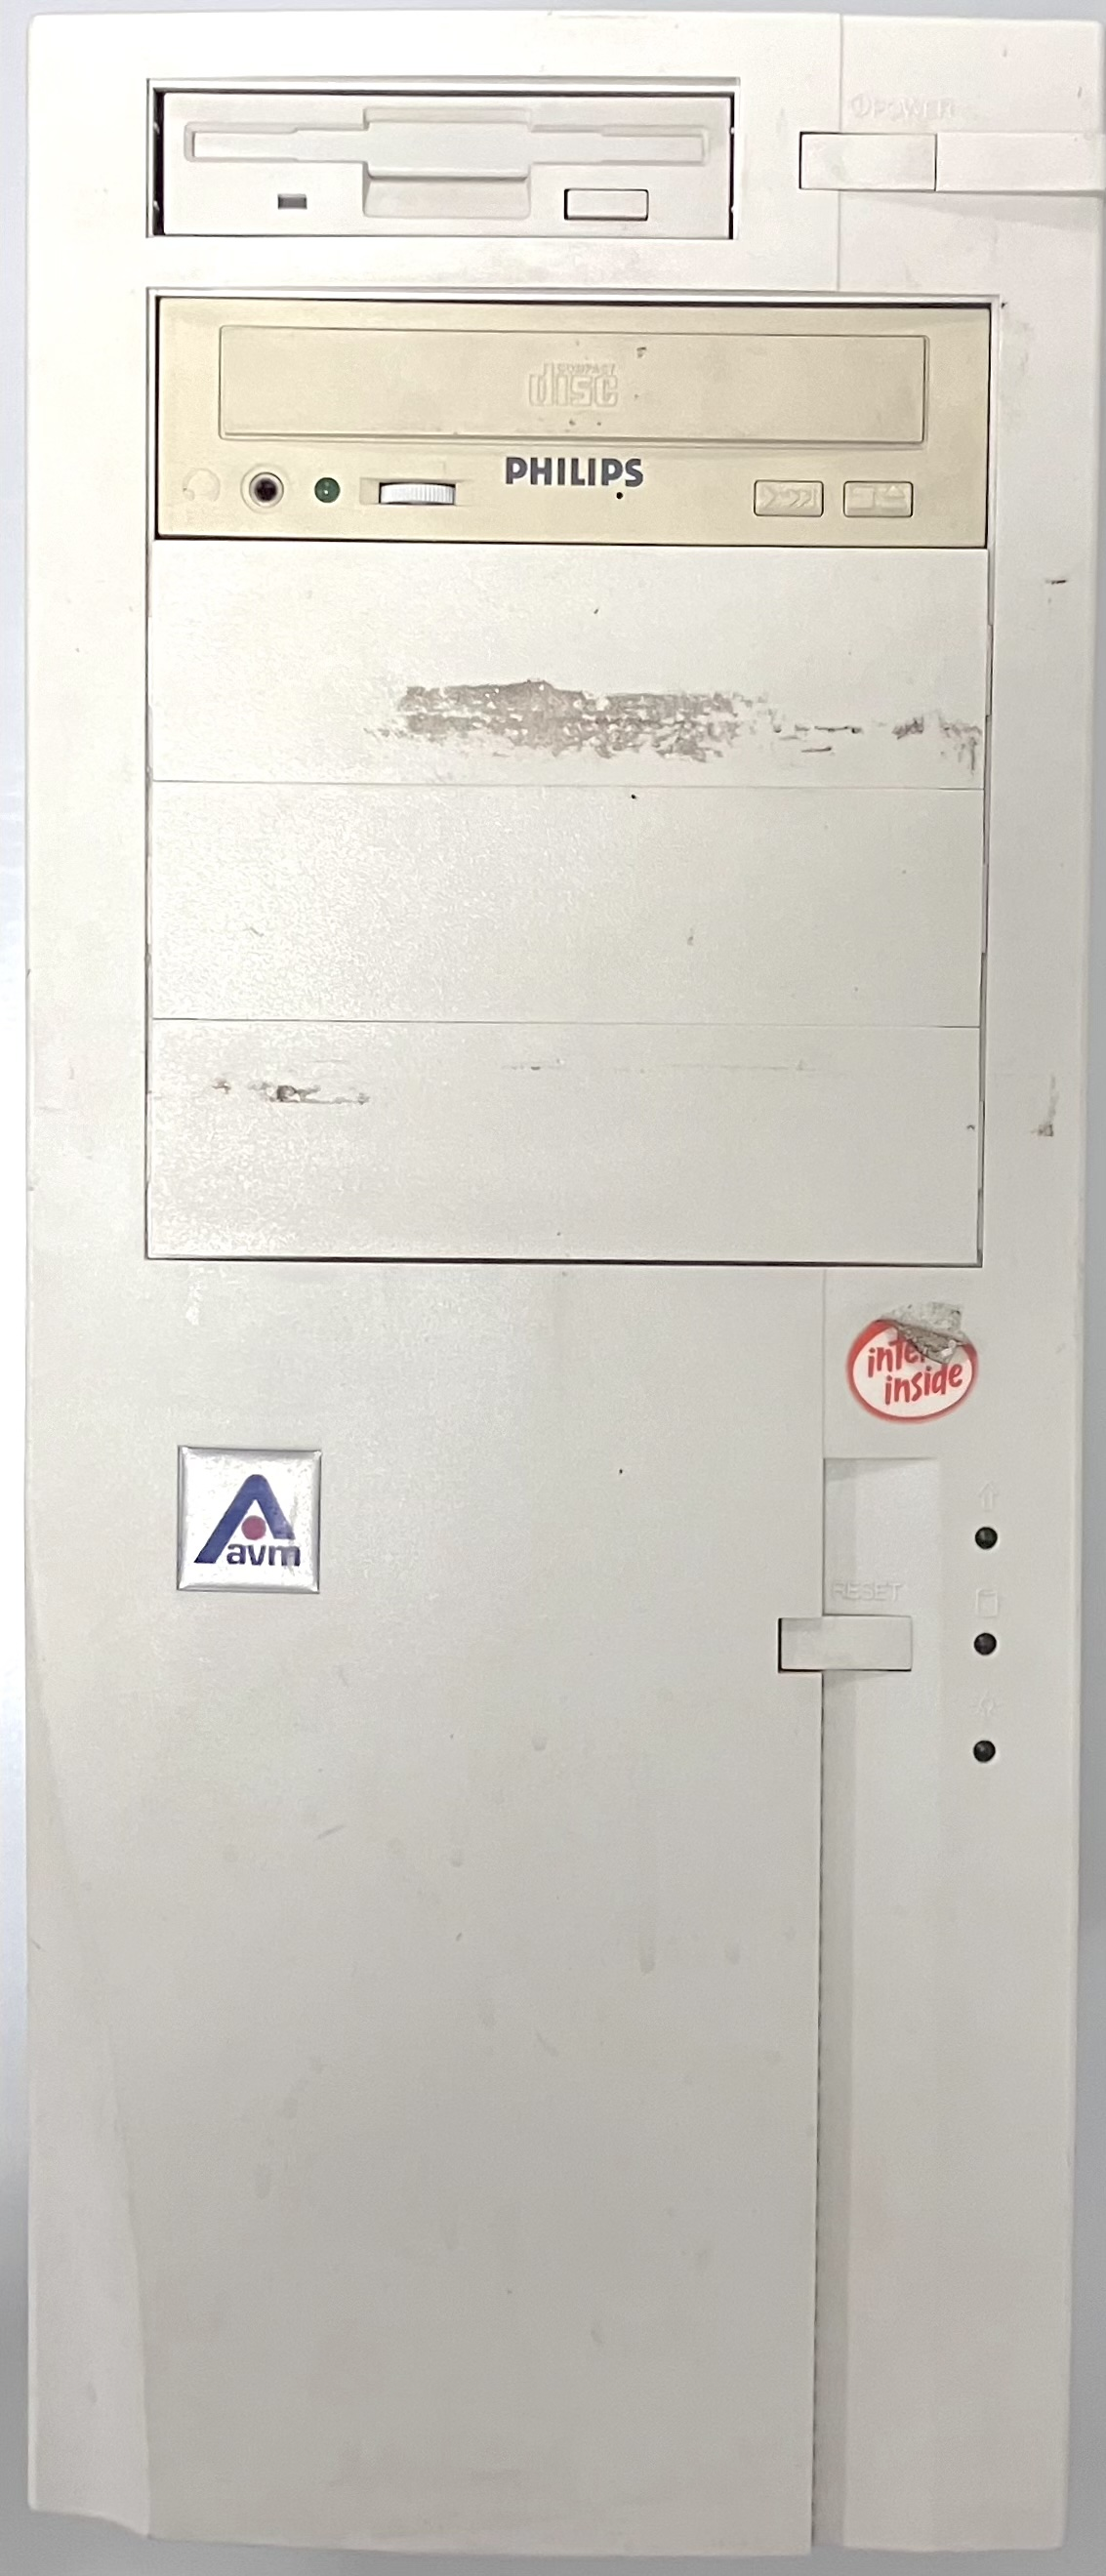
\includegraphics[width=0.75\linewidth]{chapters/appendix/b/image/figb-ilcaosdellesfere-computer012jpg.jpg}
    \end{minipage}%
    \hfill
    \begin{minipage}[t]{0.48\textwidth}
        \centering
        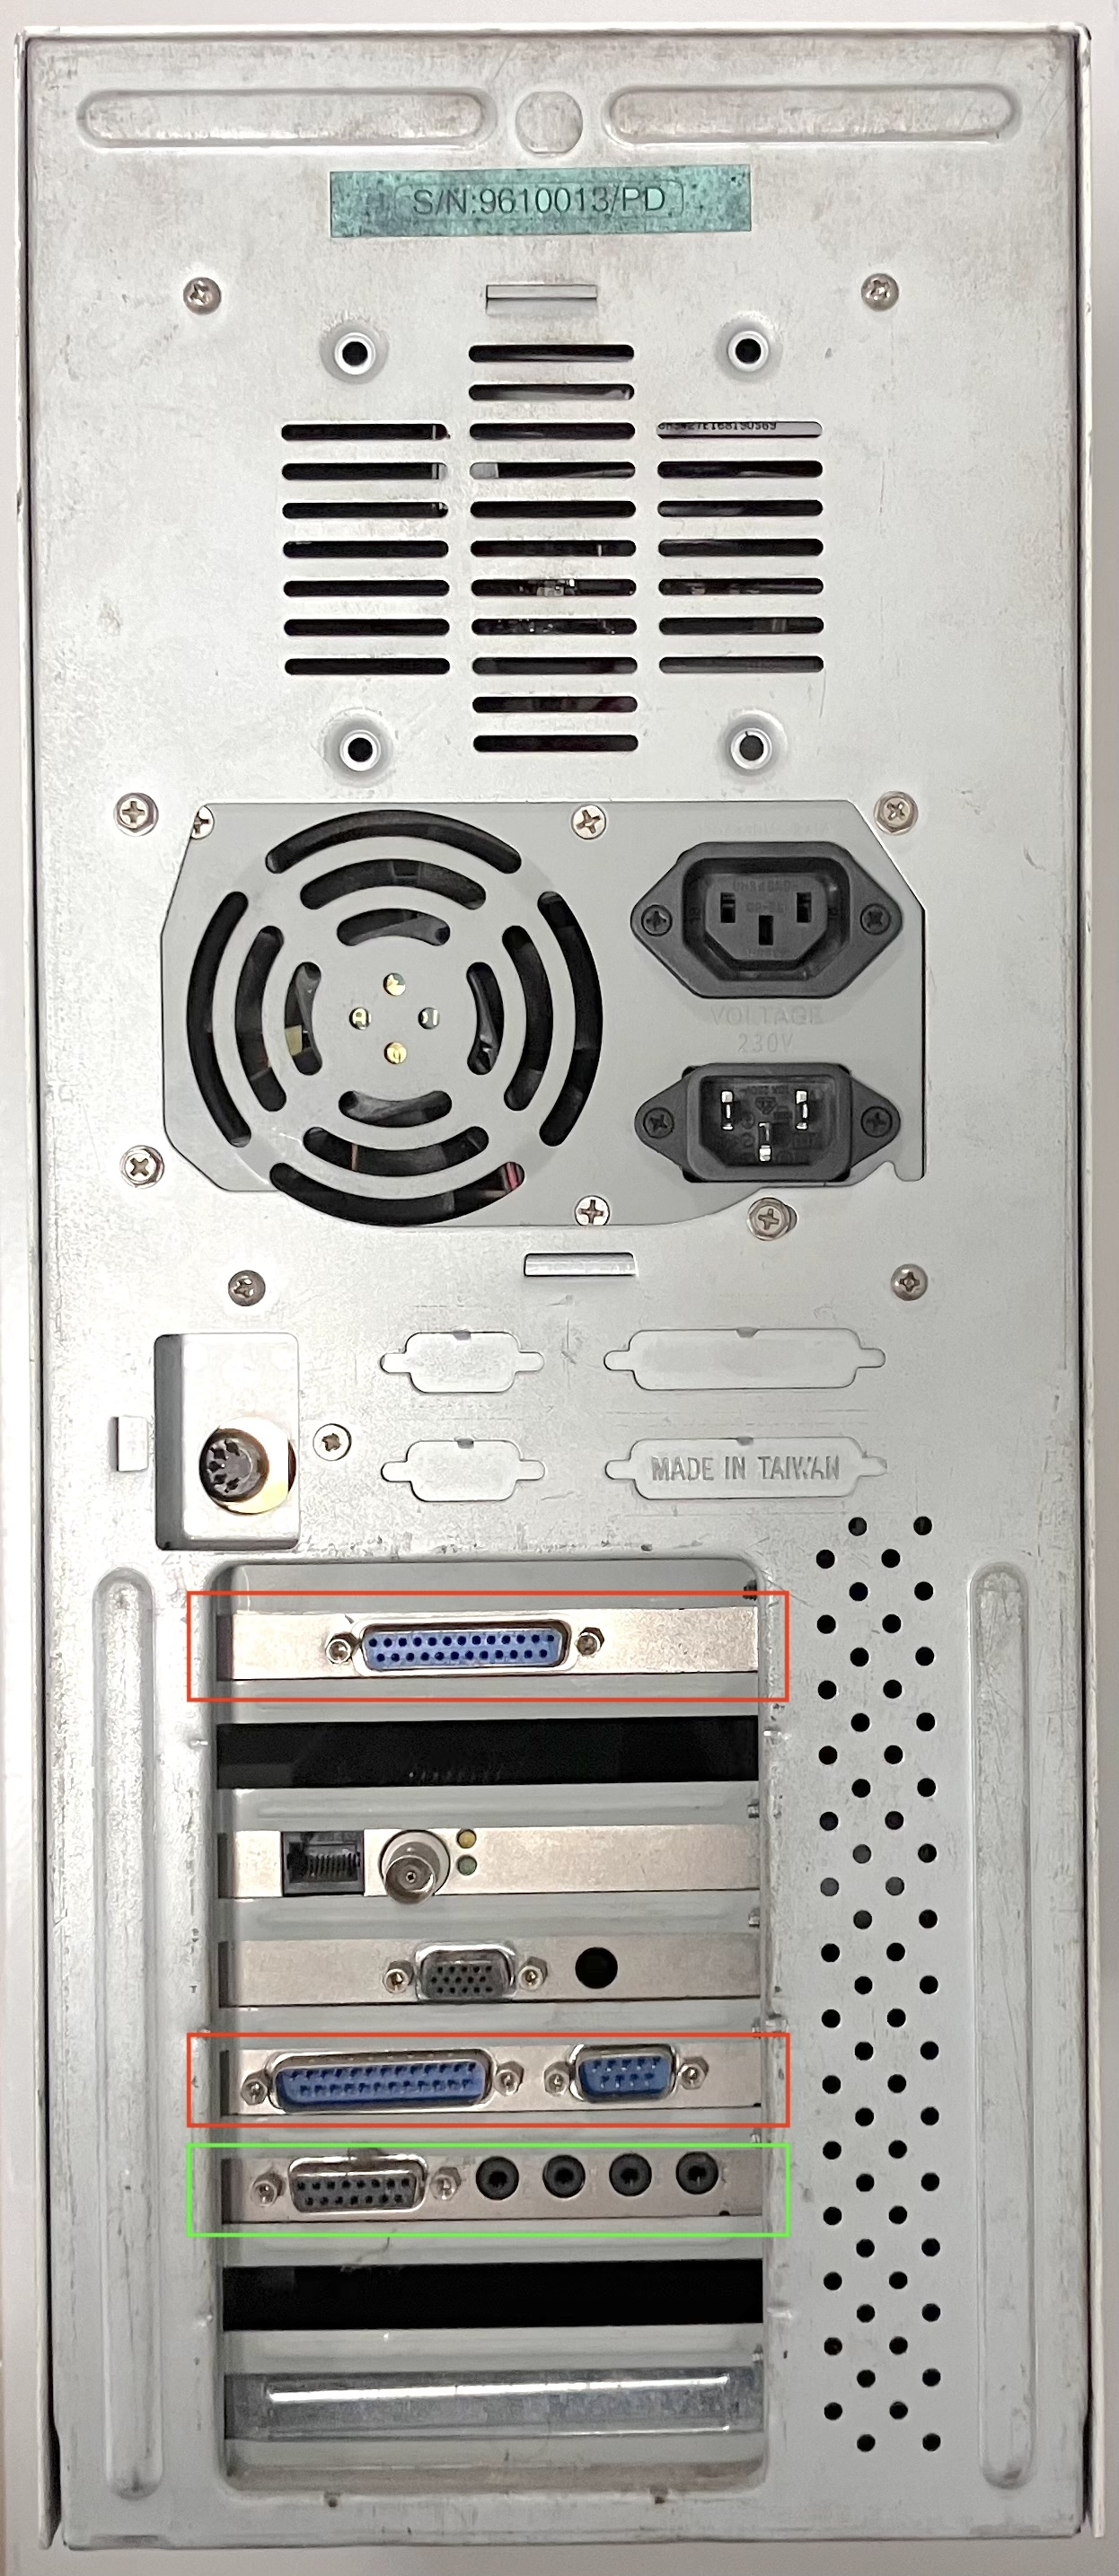
\includegraphics[width=0.75\linewidth]{chapters/appendix/b/image/figb-ilcaosdellesfere-computer01.jpg}
    \end{minipage}
    \caption{The 1998 original Desktop Personal Computer with Windows 1995. The image on the left shows the front cover, while image on the right shows the back of the computer with the damaged DB25 parallel port (within the first red rectangle), the graphical card (within the second red rectangle), and the sound card with the MIDI port (within the green rectangle).}
    \label{fig:ab-ilcaosdellesfere-computer}
\end{figure}
Additionally, the software was poorly organised and could not run on modern machines (the source code was incompatible with current systems). While the pinball machine was well preserved at the CSC laboratories and the Disklavier could still be rented or replaced, the obsolescence of the computer made it impossible to exhibit the installation again. Simply restoring the computer's old technology wasn't enough. Replacing its parts with older hardware from the time the artwork was created would only offer a short-term solution (finding compatible parts will be increasingly difficult). While the function and the physical presence of both the pinball and the Disklavier coincide, the computer presence is irrelevant –as we can deduce from the conceptual and physical implementation mappings. Only the computer’s communication function is relevant.\\
Assessing the conceptual and physical implementation mappings and the condition of the installation’s parts defined the design space for the reactivation. This space is generally determined by replacing the communication system's hardware while keeping the original elements for interaction and playback. We considered different development paths at this stage, including new hardware that could replace the original computer and run the communication function. We experimented with different paths through prototypes and evaluations.

\subsection*{Transcription}
The first step was to create a communication prototype to receive the signals sent by the pinball machine through the 25-pin parallel communication port. The main idea of the development paths was to replace the personal computer with a microcontroller or a single-board computer. Modern microcontrollers and single-board computers can easily match the performance of computers from the 1990s. We chose the Raspberry PI flagship series as single-board computers and the Arduino Mega 2560 microcontroller primarily because they offer the required number of pins—at least 25.\\
The initial communication tests were conducted using the Arduino Mega 2560, which helped us identify the type of communication involved in the installation. Indeed, parallel ports can operate in various modes, such as \textit{Compatibility Mode}, \textit{Byte Mode}, \textit{Nibble Mode}, \textit{Extended Capabilities Port Mode}, and \textit{Enhanced Parallel Port Mode}—each with different implementations, limitations, and possibilities. After these first tests, we confirmed that the installation uses \textit{Nibble Mode}, which is one of the modes capable of providing peripheral-to-host transfers. The communication with the Disklavier happens via MIDI, a simple and widely-used protocol, making its implementation much less complicated. At this point, we prototype and test simple systems (both hardware and software) to enable communication between the pinball and the Disklavier using the Arduino Mega 2560 and Raspberry PI. However, we encountered challenges when using the Raspberry PI, specifically version 3. While the parallel port sends 5V signals, the Raspberry PI works at 3.3V. Even though we used 3.3V to 5V bidirectional logic converters to balance the two systems, communication errors occurred, increasing the system's complexity. Ultimately, we decided to use the Arduino Mega 2560 microcontroller board, which provides straightforward compatibility with the DB25 parallel port interface.\\
After successfully evaluating the communication system, the final step was to port the entire source code from the C programming language to the Arduino IDE (based on C++). To understand the ``rules of the game'' (i.e., how the software processes the pinball signals and how musical events are connected to the gameplay) and perform the software porting, we conducted an in-depth analysis of the original source code. This ``archaeological'' investigation resulted in creating a high-level process mapping of the algorithm, shown in Figure~\ref{fig:ab-mapping-process}. The process mapping description significantly simplified the software porting process.\\
In the end, a working prototype of the communication node was developed to replace the original computer—Figures~\ref{fig:ab-ilcaosdellesfere-arduino} show schematics of the prototype and its realisation on a breadboard, respectively.

\begin{figure}[h!]
    \centering
    \begin{minipage}[t]{0.61\textwidth}
        \centering
        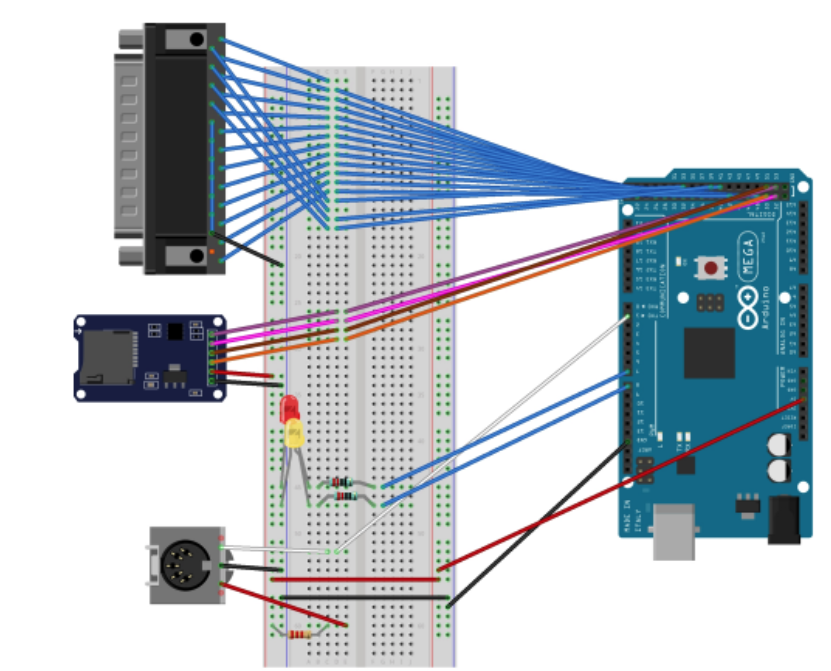
\includegraphics[width=\linewidth]{chapters/appendix/b/image/figb-ilcaosdellesfere-arduino01.png}
    \end{minipage}%
    \hfill
    \begin{minipage}[t]{0.35\textwidth}
        \centering
        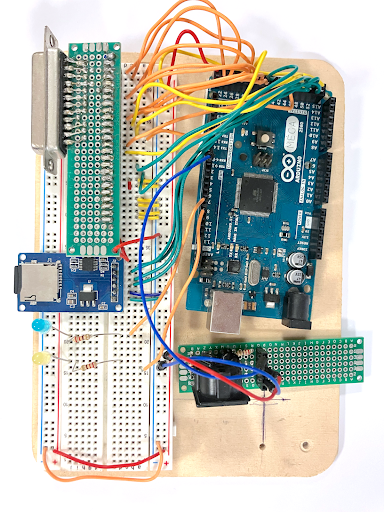
\includegraphics[width=\linewidth]{chapters/appendix/b/image/figb-ilcaosdellesfere-arduino02.png}
    \end{minipage}
    \caption{The communication node working prototype implemented on an Arduino Mega 2560 microcontroller: on the right the schematics of the prototype; on the left the working prototype created for the installation.}
    \label{fig:ab-ilcaosdellesfere-arduino}
\end{figure}

\subsection*{Transmission}
After migrating the communication node's hardware, we implemented the entire installation. The reactivated version was exhibited during the \textit{Science4all} festival (shown in Figure~\ref{fig:ab-ilcaosdellesfere-exhibition}), a scientific outreach event at the University of Padua, held on September 30, 2022 (alongside the installation of Michele Sambin's \textit{videoloop}, as described in Appendix~\ref{ax:a-michele_sambin_videoloop}).\\
Since the game allows for many possible outcomes, some situations occurred during the exhibition that had never come up in previous lab tests. These led to a few bugs in the software porting process. The bugs were fixed during the exhibition and further reviewed in the lab afterwards. This was a unique case where the redesign phase overlapped with the implementation phase. Figure~\ref{fig:ab-ilcaosdellesfere-exhibition} shows the active installation during the exhibition, highlighting the installation's key components (the computer used to manage the bugs is also visible in this image, which was taken a moment after the bug repair).\\
The current version has undergone further optimisations and runs in the CSC lab.

\begin{figure}[!h]
    \centering
    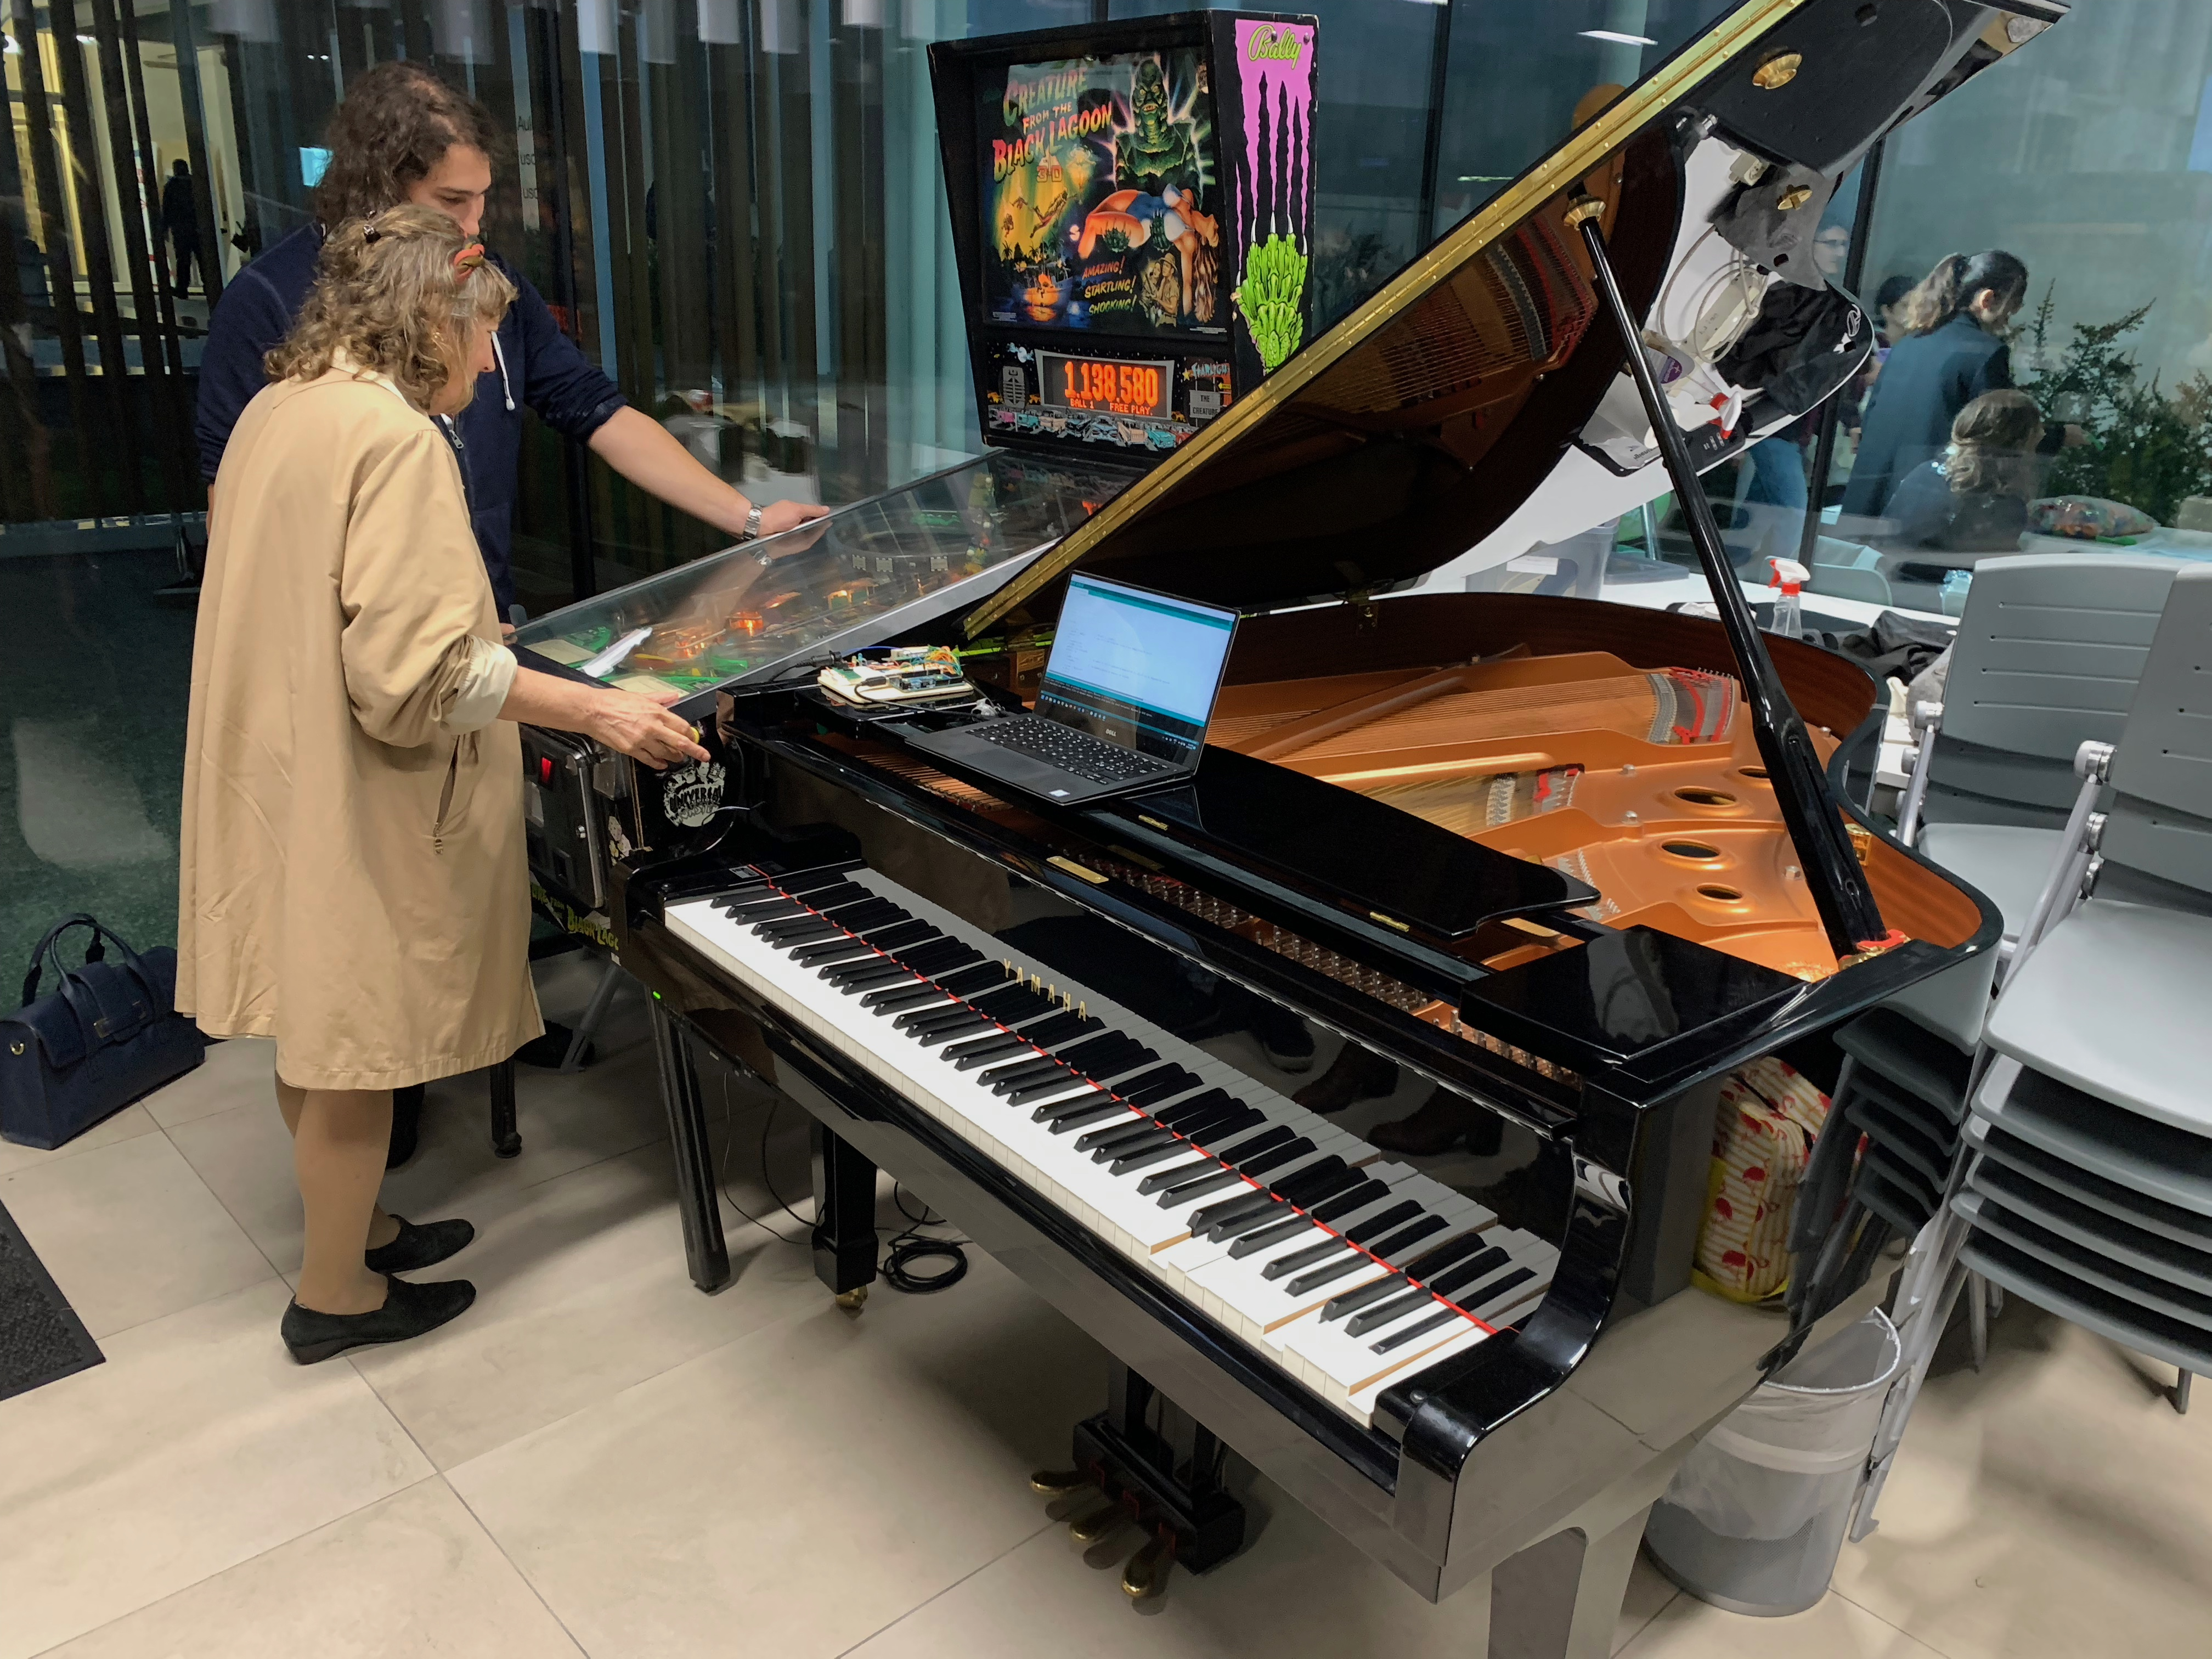
\includegraphics[width=\linewidth]{chapters/appendix/b/image/figb-ilcaosdellesfere-exhibition.jpg}
    \caption{ The interactive installation \textit{Il caos delle sfere} reactivated and exhibited during the University of Padua’s \textit{Science4all} festival on September 30, 2022.}
    \label{fig:ab-ilcaosdellesfere-exhibition}
\end{figure}

\subsection*{Archiving}
All the \textit{bit}s, \textit{data}, and \textit{experience}s produced during the reactivation process were stored and organised as a new \textit{Iteration File} (IF) according to the MDC model.\\ 
Most of the \textit{bit}s (Pinball and Disklavier) remain unchanged compared to the first IFs. At the same time, the computer and its related software (the \textit{communication node}) have been migrated, creating a new entry.\\ 
In addition, the new IF includes all the instructions, which are composed of \textit{conceptual}, \textit{physical implementation}, and \textit{process mappings}. This information is essential to reactivate the installation and port the software again, if necessary. The \textit{conceptual} (Figure~\ref{fig:ab-mapping-conceptual}) and high-level \textit{process} (Figure~\ref{fig:ab-mapping-conceptual}) mappings are created and used in this reactivation and belong to the new IF. However, since they have been developed as descriptions of the previous iterations (which missed the data part), they can also belong to them through \textit{multiple belongingness} (as shown in Figure~\ref{dafare}). \\
Finally, photos and audiovisual documentation were produced during the \textit{assessment}, \textit{transcription}, and \textit{transmission} phases, which have been recorded as \textit{experience}-type items in the new IF.\\
All the documentation of \textit{Il caso delle sfere} has been archived using the Neo4j graphical databse, as explained in Chapter~\ref{ch:4-madc_model_application}.

\section{Data compilation}
We report some of the most essential parts of the technical instructions and mappings based intruction template introduced in Chapter~\ref{ch:3-mdc_model-reactivation_workflow-instruction_template} and Chapter~\ref{ch:4-madc_model_application}.

\subsection*{Bit list and specifications}
The table reports the list of \textit{bit}s divided by hardware, software, and files. We can separate the hardware list into two different sections: \textit{implementation} and \textit{development}. The \textit{implementation} section specifies the main \textit{bit}s used for setting the installation up; the \textit{development} section can also be compiled to describe the component used to construct the single main \textit{bit}s, e.g., the component used for creating \textit{Il caos delle sfere Communication Node }(ICDS-CN) computer.

\begin{longtable}{|p{0.3\textwidth}|p{0.05\textwidth}|p{0.55\textwidth}|}
    \caption{Hardware (Implementation)} \label{tab:a-data-hardware} \\
    \hline
    \textbf{Name} & \textbf{Q} & \textbf{Specification and notes} \\
    \hline
    Creature from the Black Lagoon Pinball & 1 & \scriptsize Mechanical Pinball with the self-built PCB for sending the sensors’ signal through the parallel port.\\
    \hline
    Disklavier & 1 & \scriptsize Any Disklavier models can be used without any specific limitation. Both upright or grand piano Disklavier can used.  \\
    \hline
    ICDS-CN computer & 1 & \scriptsize Self-built microcontroller computer that converts the pinball signal into MIDI musical sequences according to Carlo De Pirro’s instructions. \\
    \hline
    Micro SD & 1 & \scriptsize $\geq$ 256MB \\
    \hline
    25-pin Parallel cable  & 1 & \scriptsize \\
    \hline
    MIDI cable & 1 & \scriptsize \\
    \hline
\end{longtable}

\begin{longtable}{|p{0.3\textwidth}|p{0.05\textwidth}|p{0.55\textwidth}|}
    \caption{Hardware (Development)} \label{tab:a-data-hardware} \\
    \hline
    \textbf{Name} & \textbf{Q} & \textbf{Specification and notes} \\
    \hline
    Microcontroller & 1 & \scriptsize Operating Voltage: 5V; Digital I/O Pins: $\geq$ 22; PWM Pins out: $\geq$ 2 (only for debugging); TX0 pin: $\geq$ 1; \textbf{Suggested}: Arduino Mega 2560.\\
    \hline
    MIDI port & 1 & \scriptsize With related resistors (usually two 220$\Omega$).\\
    \hline
    MicroSD Card Module & 1 & \scriptsize \textbf{Suggested}: CATALEX Micro SD Card Module\\
    \hline
    DB25 port (female) & 1 & \scriptsize \\
    \hline
    Led  & 2 & \scriptsize (Only for debugging) different colours and the related resistors.  \\
    \hline
    Jumpers & $\sim$40 & \scriptsize \\
    \hline
    USB-B cable & 1 & \scriptsize For deploying the firmware or debugging. \\
    \hline
\end{longtable}

\begin{longtable}{|p{0.35\textwidth}|p{0.55\textwidth}|}
    \caption{Software} \label{tab:a-data-hardware} \\
    \hline
    \textbf{Name} & \textbf{Specification and notes} \\
    \hline
    ICDS-CN firmware & \scriptsize \\
    \hline
    Arduino IDE & \scriptsize Version 1.8. For uploading the firmware.\\
    \hline
    SPI Arduino IDE library & \scriptsize Communication with the Micro SD Card Module will be via SPI protocol.  \\
    \hline
    SD Arduino IDE library & \scriptsize To access, read, and write the SD card.\\
    \hline
\end{longtable}

\begin{longtable}{|p{0.35\textwidth}|p{0.55\textwidth}|}
    \caption{File} \label{tab:a-data-hardware} \\
    \hline
    \textbf{Name} & \textbf{Specification and notes} \\
    \hline
    sqnz.txt & \scriptsize MIDI note sequences text file (uploaded on the SD card).\\
    \hline
    acc1.txt & \scriptsize MIDI note sequences text file (uploaded on the SD card).  \\
    \hline
    acc2.txt & \scriptsize MIDI note sequences text file (uploaded on the SD card).\\
    \hline
    ICDS-CN.ino & \scriptsize source code for the ICDS-CN firmware.\\
    \hline
\end{longtable}

\subsection*{Conceptual mapping}
Figure~\ref{fig:ab-mapping-conceptual} shows the \textit{conceptual mapping} of the \textit{Il caos della sfere} interactive installation made with the BVL. The main concept of this installation is the audience interacting by playing the increasingly complex pinball game, which results in the Disklavier playing more or less complex musical sequences.

\begin{figure}[!h]
    \centering
    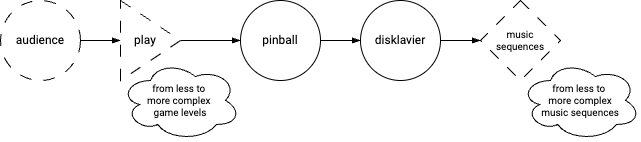
\includegraphics[width=\linewidth]{chapters/appendix/b/image/graphb-mapping-concept.png}
    \caption{\textit{Il caos delle sfere}’s \textit{Conceptual mapping} with BVL.}
    \label{fig:ab-mapping-conceptual}
\end{figure}

\subsection*{Physical implementation mapping}
Figure~\ref{fig:ab-mapping-physical} shows a \textit{physical implementation mapping} of the first versions of \textit{Il caos delle sfere}, which can be extended to Figure~\ref{fig:ab-mapping-physical02}, including the self-built PCB for communicating through parallel ports. The representation in Figure~\ref{fig:ab-mapping-physical} helps better distinguish between the main \textit{bit}s according to their specific functions (\textit{interaction}, \textit{communication}, and \textit{playback}).

\begin{figure}[!h]
    \centering
    
\includegraphics[width=\linewidth]{chapters/appendix/b/image/graphb-mapping-physical01.png}
    \caption{\textit{Il caos delle sfere} past versions’ \textit{physical implementation mapping} with BVL.}
    \label{fig:ab-mapping-physical}
\end{figure}

\begin{figure}[!h]
    \centering
    
\includegraphics[width=\linewidth]{chapters/appendix/b/image/graphb-mapping-physical02.png}
    \caption{Extension of \textit{Il caos delle sfere} past versions’ \textit{physical implementation mapping}, including the self-built PCB.}
    \label{fig:ab-mapping-physical02}
\end{figure}

Figure~\ref{fig:ab-mapping-physical03} shows the \textit{physical implementation mapping} of the reactivated version of \textit{Il caos delle sfere}. 

\begin{figure}[!h]
    \centering
    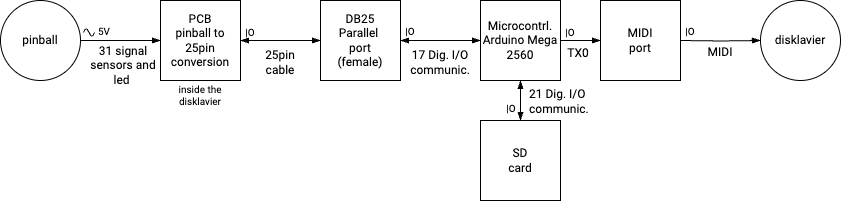
\includegraphics[width=\linewidth]{chapters/appendix/b/image/graphb-mapping-physical03.png}
    \caption{\textit{Il caso delle sfere} reactivation’s \textit{physical implementation mapping} with BVL.}
    \label{fig:ab-mapping-physical03}
\end{figure}

\subsection*{Process mapping}
Figure~\ref{fig:ab-mapping-process} reports the \textit{process mapping}'s highest level of the \textit{Il tempo consuma software}, developed from the old implementations and used to port the code to the C++ programming language in Arduino IDE.
\begin{figure}[!h]
    \centering
    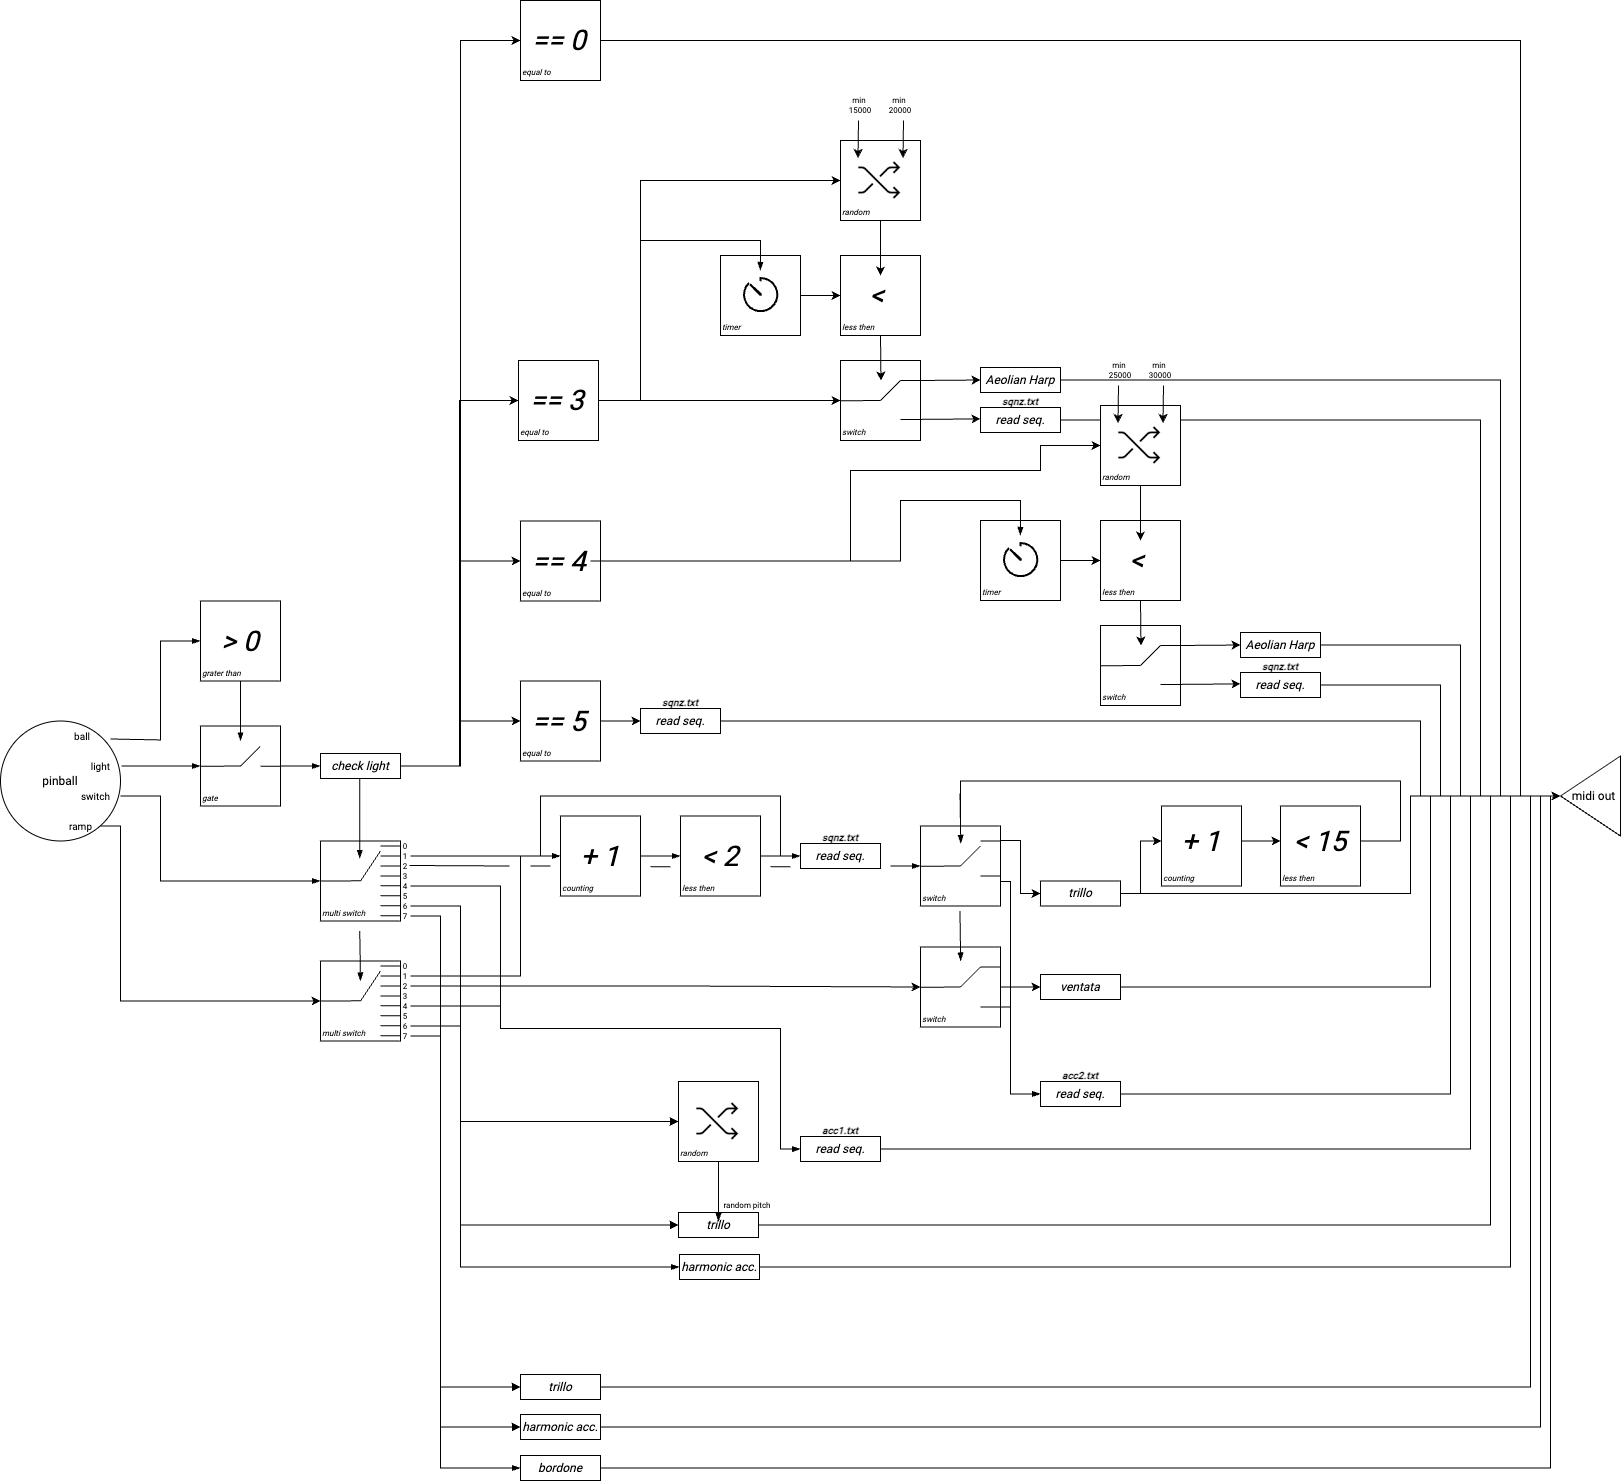
\includegraphics[width=\linewidth]{chapters/appendix/b/image/graphb-mapping-process.png}
    \caption{\textit{Il caso delle sfere} reactivation’s high-level \textit{process mapping}. The rectangular boxes (e.g. trillo, read seq., etc.) represent specific \textit{Functions} in the code, which are described through other process mappings (as also explained in Chapter~\ref{ch:4-madc_model_application}).}
    \label{fig:ab-mapping-process}
\end{figure}

\section{Results and discussion}
This case study enabled a crucial distinction between the core elements of interactive installations, identifying two types: ``elements of the experience'' and ``elements for the experience''. The first type represents the visible components, the ``surface'' of the work, which the audience encounters directly through various sensory levels. For example, in \textit{Il caos delle sfere}, these elements include the pinball machine and the Disklavier, which the audience interacts with through play and music. The second type involves elements that operate indirectly (in the sense that they are activated as a result of an action of audiences or performers and act as a cause for feedback), driving the experience by providing the ``logic'' of the artwork. These components shape and activate the ``elements of the experience'' according to the installation's ``rules.'' In \textit{Il caos delle sfere}, examples include the computer and software that connect the pinball machine and Disklavier, determining how specific game events trigger musical responses.This distinction also emerges from overlapping the different descriptive levels of the artwork. For instance, comparing conceptual mapping (Figure~\ref{fig:ab-mapping-conceptual}) and physical implementation (Figure~\ref{fig:ab-mapping-physical}) reveals that while the computer is not part of the conceptual level, it is essential for realising the installation\footnote{The distinction between the ``elements of the experience'' and the ``element for the experience'' is not always clear-cut as in the case of \textit{Il caos delle sfere}. These two types of elements can overlap.}.\\ 
This perspective leads to significant insights about the artwork's reactivation and enables us to move beyond common preservation strategies such as philological preservation, migration, emulation, and reinterpretation. Rather than seeing these approaches as applied to the entire artwork, we view them as methods best suited to specific elements within the artwork. In this context, we define the reactivation of \textit{Il caos delle sfere} as a \textit{hybrid reactivation}, combining a philological approach and technological migration within a single reconstruction and implementation process. This approach allows us to consider each component based on its role in the experience, thus adapting common preservation strategies to suit the unique needs of interactive installations.\\
Another interesting aspect that emerged during the exhibition was how the experience of specific technologies changes over time. People interact with the artwork through a unique instrument—the pinball machine. Specifically, \textit{The Creature from the Black Lagoon} pinball machine is an essential part of the experience, at the ``surface'' of the artwork, and plays a critical role in engaging the audience. However, this machine now evokes a strong sense of the past. When the artwork was created and premiered in the 1990s, pinball machines were common in public spaces, a familiar and accessible interface for most people. The composer chose the pinball machine as an interface precisely because it was widely recognisable and engaging at the time. Today, however, pinball machines are rare. Now, that familiarity has shifted: the pinball machine evokes memories or nostalgia for older visitors, while for younger generations—who may have never used one—it’s a novelty. Thus, reactivating this artwork introduces a new experience. Though the use of the pinball machine is faithful to the original concept, it now introduces an inevitable difference. As a result, the audience's focus has shifted. Instead of emphasising the interaction between the game and the music, the pinball machine draws attention as a historical object, altering how people experience the artwork today.\\

\begin{figure}[!h]
    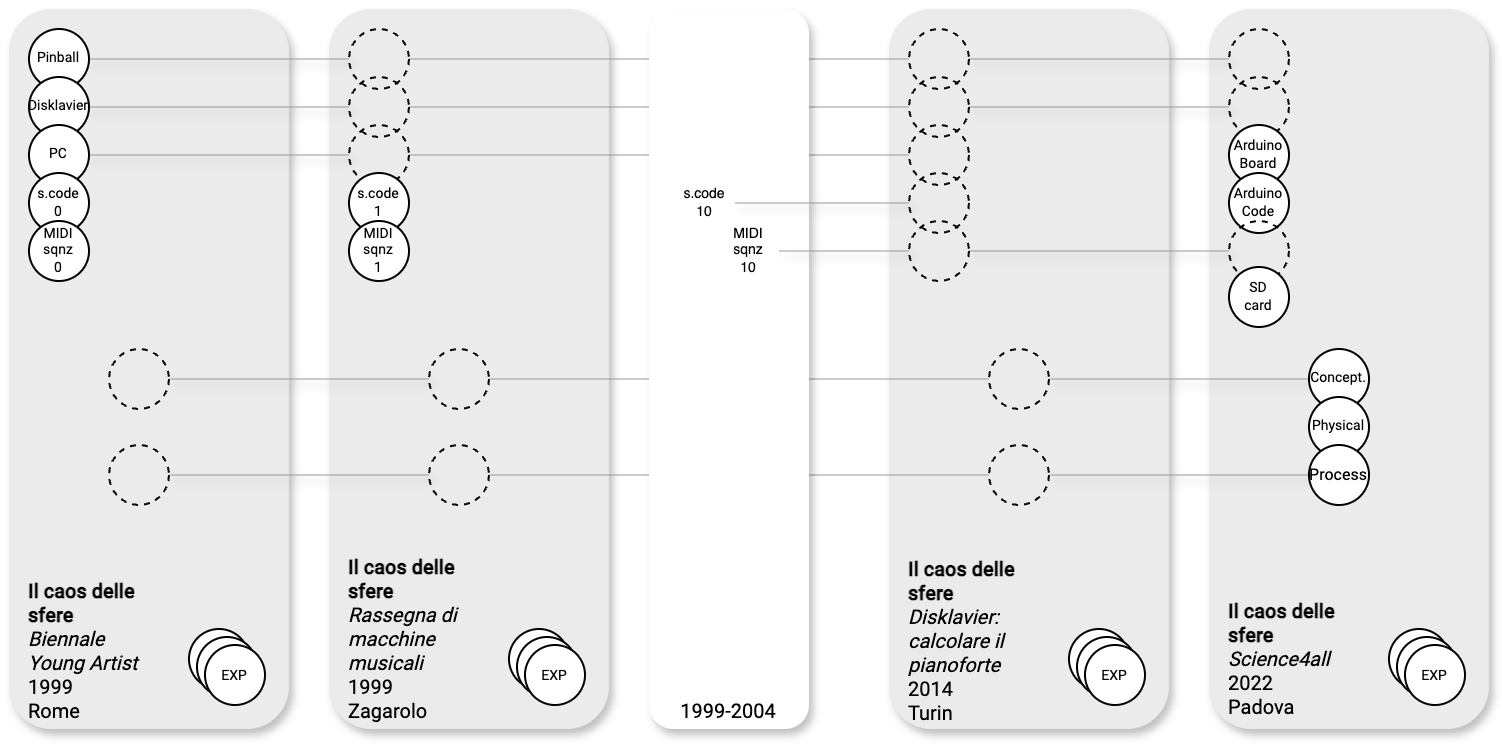
\includegraphics[width=\linewidth]{chapters/appendix/b/image/graphb-mdc.png}
    \caption{Approximate chronological representation of \textit{Il caos delle sfere} according to the MDC model. The \textit{multiple belongingness} shows the component elements that remain unchanged (e.g., Pinball) and those that change reactivation after reactivation (e.g., source code). The Figure shows that the mappings of the system were never produced until the last reactivation.}
    \label{fig:ab-graph_mdc}
\end{figure}

Figure~\ref{fig:ab-graph_mdc} shows an approximate representation of \textit{Il caos delle sfere} through the MDC Model. The \textit{multiple belongingness} shows the \textit{bit}s elements that remain unchanged (e.g., Pinball) and those that change reactivation after reactivation (e.g., source code). The figure shows that the system's \textit{data} elements were never produced until the last reactivation. Indeed, the \textit{data} item belongs to the new reactivation but is also related to the previous one through the \textit{multiple belongingness} since they have been developed as descriptions of the previous iterations.\\
Finally, experience elements are recorded for each reactivation to document and contextualise it. This representation clearly shows how the model records the artwork's dynamic authenticity and technological history through \textit{multiple belongingness}. 

